\documentclass[tikz,border=2pt]{standalone}
\renewcommand{\familydefault}{\sfdefault}
\usetikzlibrary{arrows.meta,calc,positioning}
\tikzset{every picture/.style={line width=1pt, >=Stealth},
         hl/.style={fill=black, fill opacity=0.12, text opacity=1}}
\begin{document}
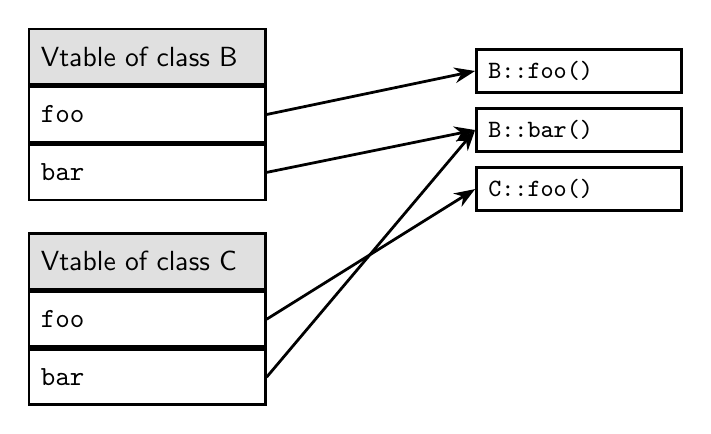
\begin{tikzpicture}[row/.style={draw, minimum width=3cm, minimum height=0.7cm, text width=2.7cm, align=left},
    fn/.style={draw, minimum width=2.6cm, minimum height=0.55cm, font=\ttfamily\small, text width=2.3cm, align=left}]
  % \vtable{name}{x}{y}{title}: a header row and one row per virtual function
  \newcommand{\vtable}[4]{
    \node[row, hl, anchor=north west] (#1) at (#2, #3) {#4};
    \node[row, below=0pt of #1] (#1foo) {\texttt{foo}};
    \node[row, below=0pt of #1foo] (#1bar) {\texttt{bar}};
  }
  \foreach \f [count=\k] in {B::foo(), B::bar(), C::foo()} \node[fn] (f\k) at (7, 0.2 - 0.75*\k) {\f};
  \vtable{B}{0}{0}{Vtable of class B}
  \vtable{C}{0}{-2.6}{Vtable of class C}
  \draw[->] (Bfoo.east) -- (f1.west);
  \draw[->] (Bbar.east) -- (f2.west);
  \draw[->] (Cfoo.east) -- (f3.west);
  \draw[->] (Cbar.east) -- (f2.west);
\end{tikzpicture}
\end{document}
